\section{Multi agent experiments}
The complexity of the problem disallow us from using a more complex model (double integrator, 1 input memory model) for multi agent scenarios.
Therefore, the $N$ quadricopters will be modelled as a $2N$ dimensions single integrators.

The quadricopters have to verify the following LTL formula:
$$ \varphi = (\LTLalways \neg out) \and (\LTLalways \LTLeventually a) \and (\LTLalways \LTLeventually b) \and (\LTLalways \neg collide)$$
where $out$ correspond to one quad or more outside of the environment, $a$ agent 1 in north-east and agent 2 in south-west, $b$ agent 1 in south-west and agent 2 in north-east and $collide$ if there is a collision (quads on the same cells).
Figure \ref{fig:multi} show a run of the plan for few steps.



\begin{figure}
  \newcommand*\FigVSkip{0.5em}
  \newcommand*\FigHSkip{0.1em}
  \newsavebox\FigBox
  \centering
  % Top image is centered, so no need to get width
  \begin{minipage}{0.3\textwidth}
    \centering
    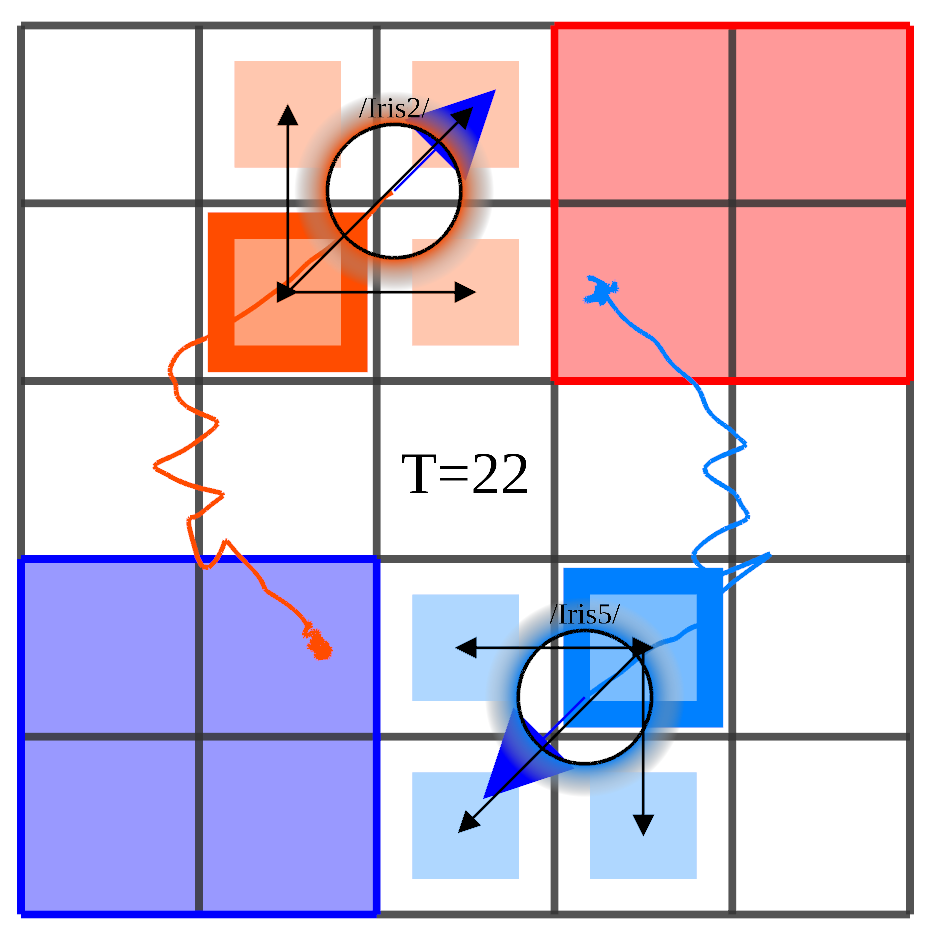
\includegraphics[width=\linewidth]{multi_ltl/multi1}
  \end{minipage} 
  \begin{minipage}{0.3\textwidth}
    \centering
    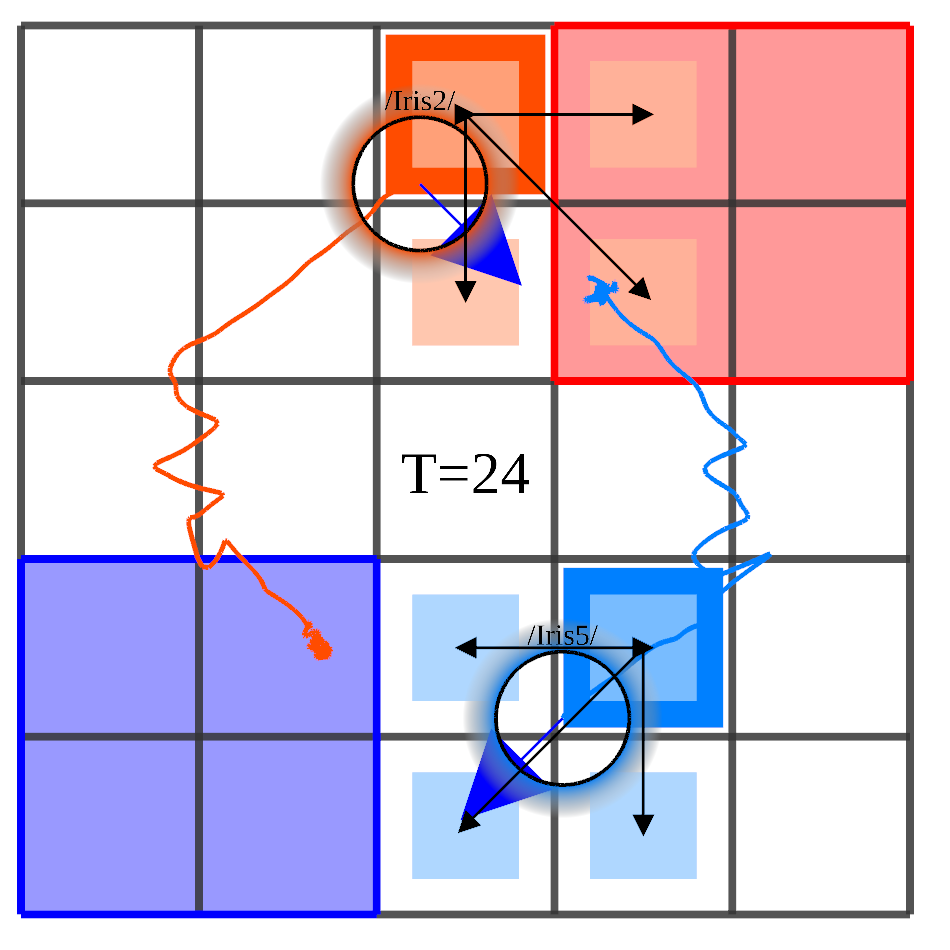
\includegraphics[width=\linewidth]{multi_ltl/multi2}
  \end{minipage} 
  \begin{minipage}{0.3\textwidth}
    \centering
    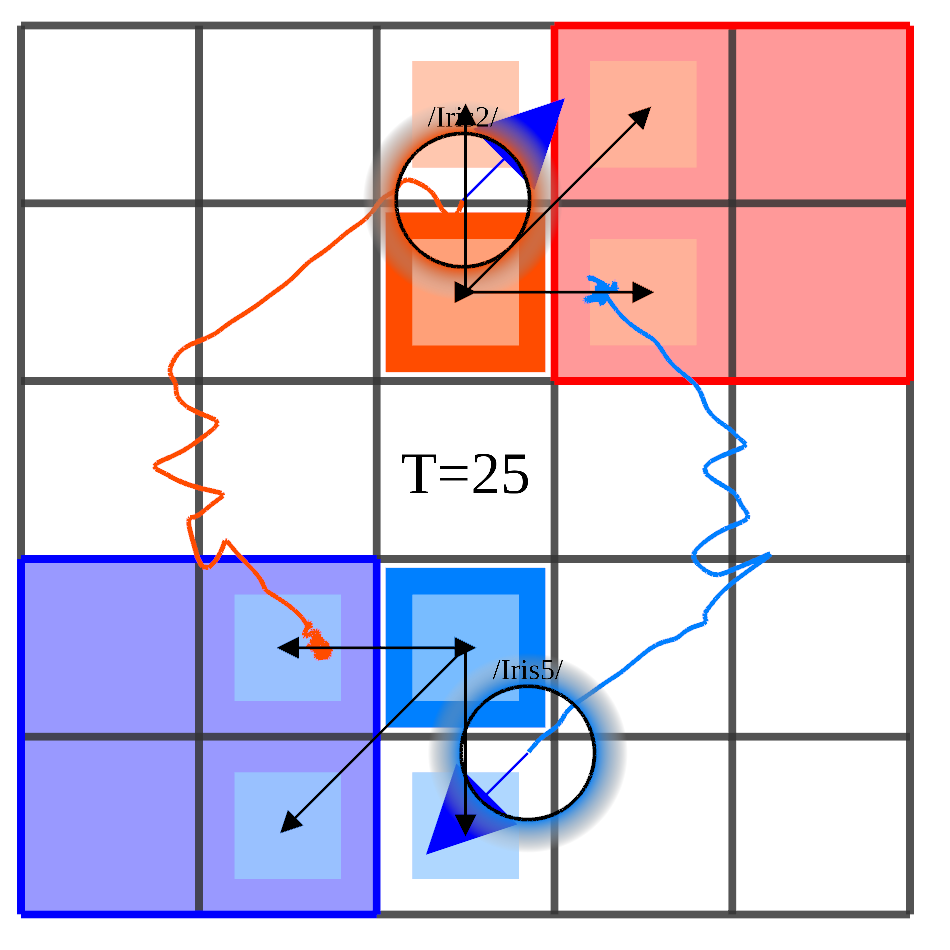
\includegraphics[width=\linewidth]{multi_ltl/multi3}
  \end{minipage} 
  \\[\FigVSkip]%
  % Top image is centered, so no need to get width
  \begin{minipage}{0.3\textwidth}
    \centering
    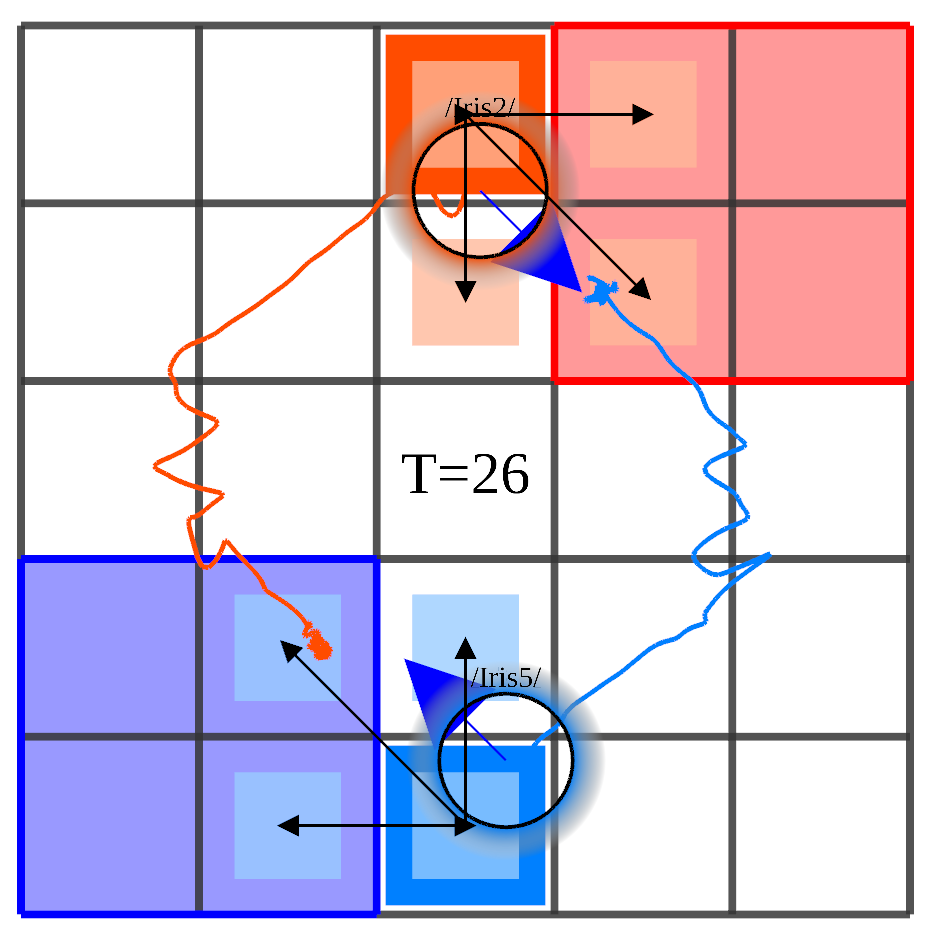
\includegraphics[width=\linewidth]{multi_ltl/multi4}
  \end{minipage} 
  \begin{minipage}{0.3\textwidth}
    \centering
    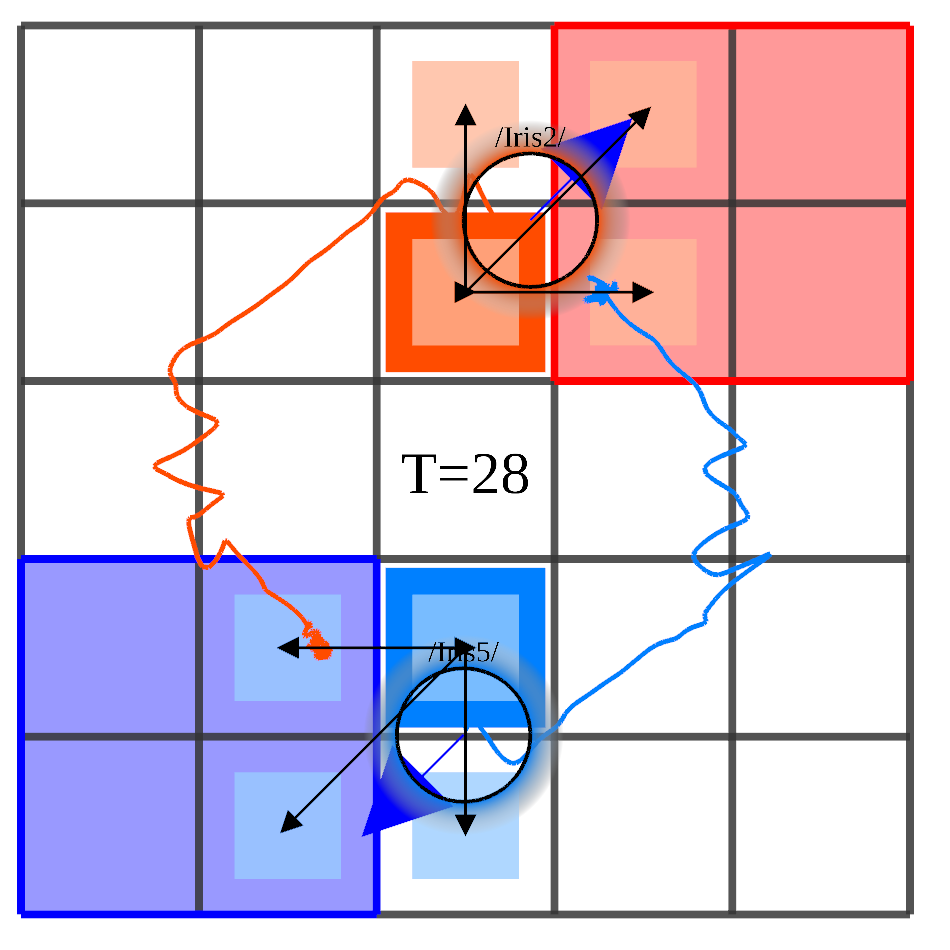
\includegraphics[width=\linewidth]{multi_ltl/multi5}
  \end{minipage} 
  \begin{minipage}{0.3\textwidth}
    \centering
    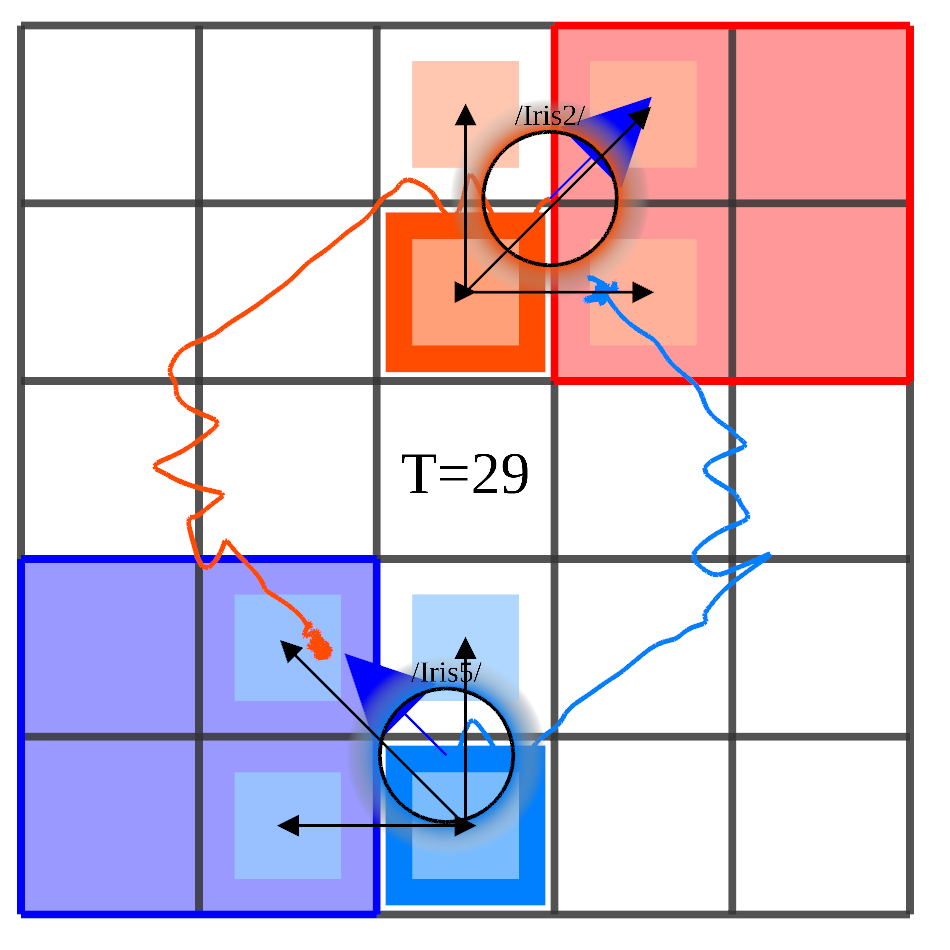
\includegraphics[width=\linewidth]{multi_ltl/multi6}
  \end{minipage} 
  \\[\FigVSkip]%
  % Top image is centered, so no need to get width
  \begin{minipage}{0.3\textwidth}
    \centering
    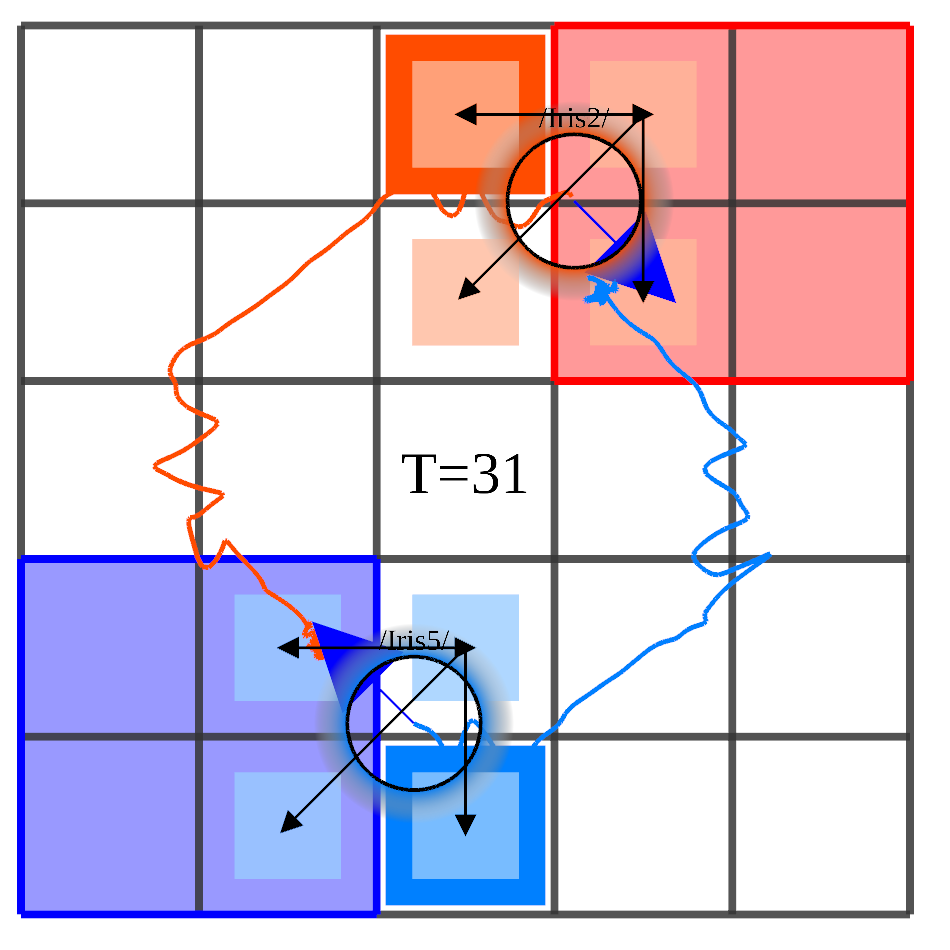
\includegraphics[width=\linewidth]{multi_ltl/multi7}
  \end{minipage} 
  \begin{minipage}{0.3\textwidth}
    \centering
    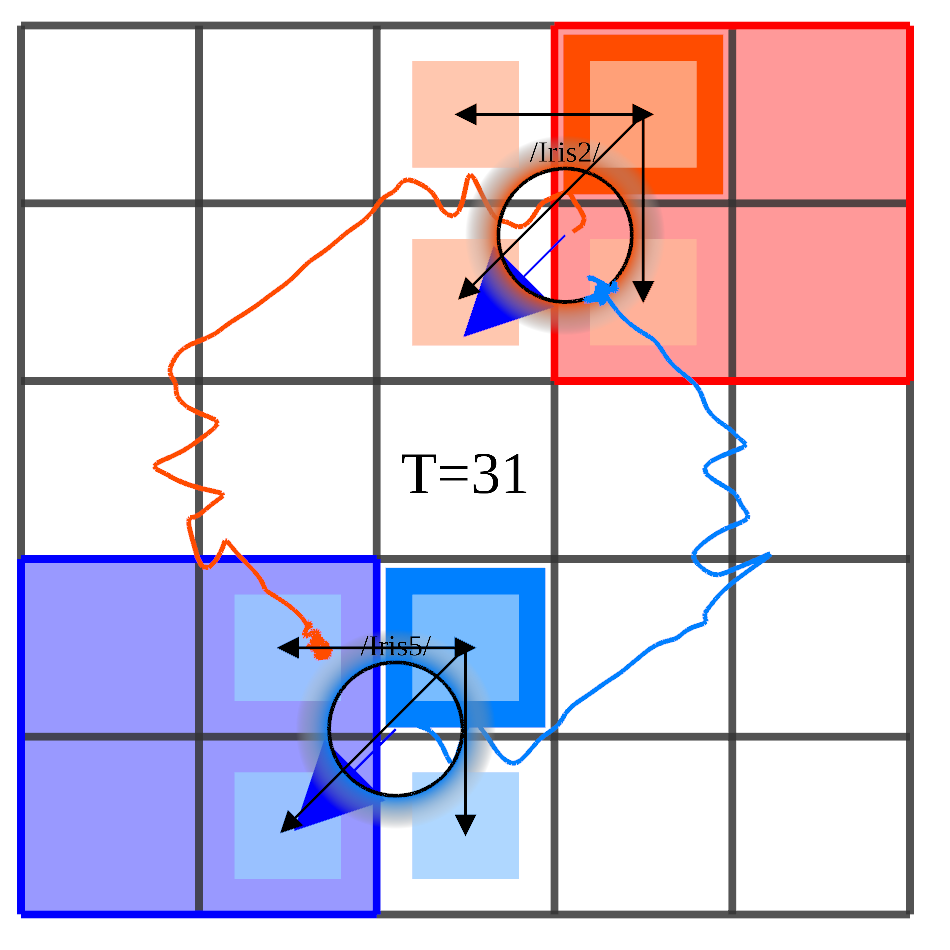
\includegraphics[width=\linewidth]{multi_ltl/multi8}
  \end{minipage} 
  \begin{minipage}{0.3\textwidth}
    \centering
    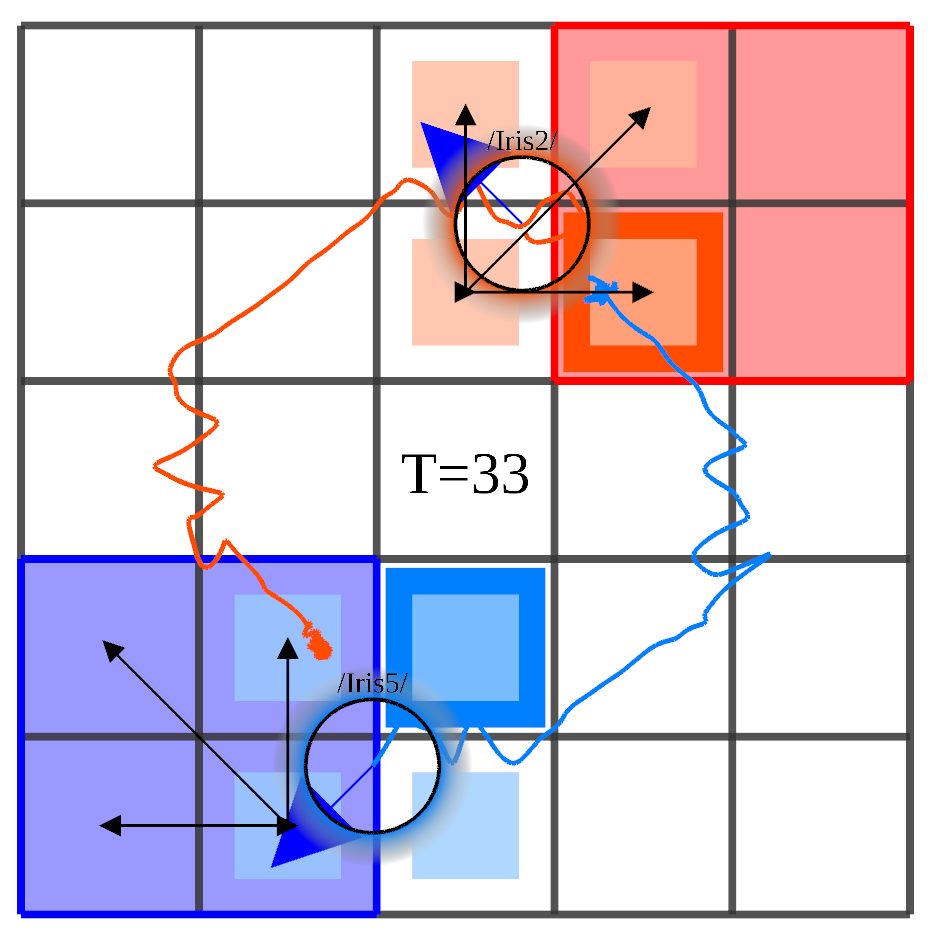
\includegraphics[width=\linewidth]{multi_ltl/multi9}
  \end{minipage} 
  \\[\FigVSkip]%
  % Top image is centered, so no need to get width
  \begin{minipage}{0.3\textwidth}
    \centering
    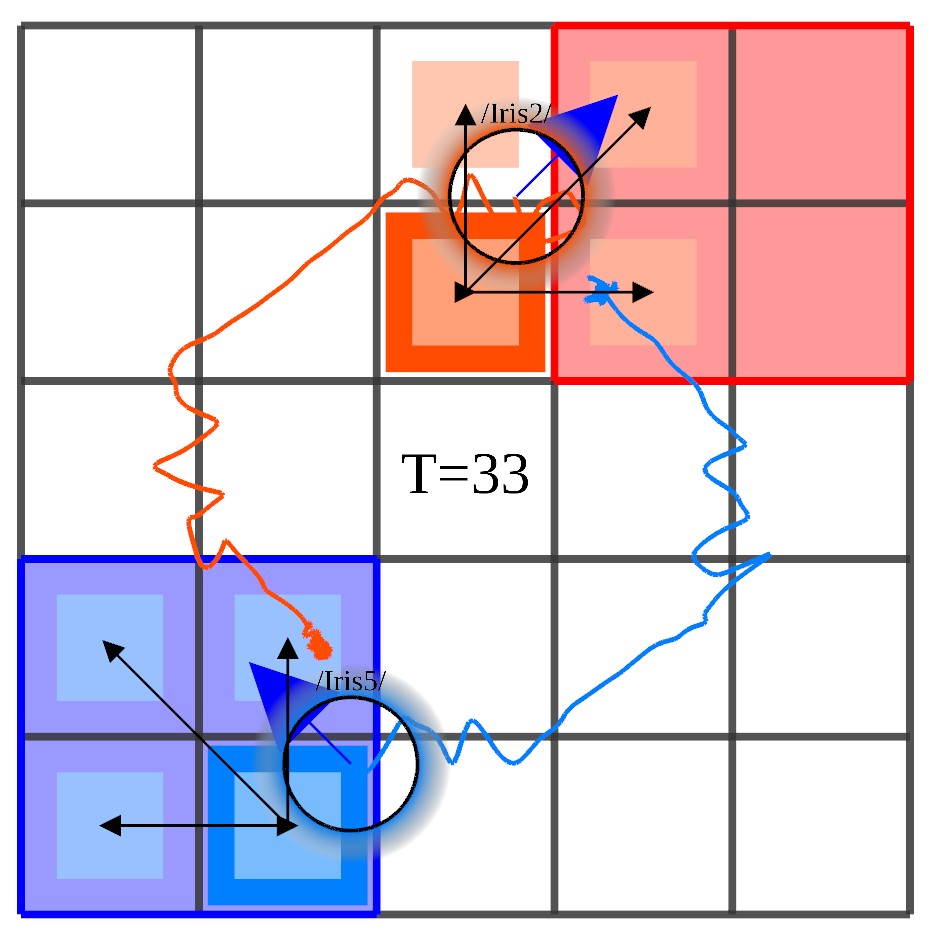
\includegraphics[width=\linewidth]{multi_ltl/multi10}
  \end{minipage} 
  \begin{minipage}{0.3\textwidth}
    \centering
    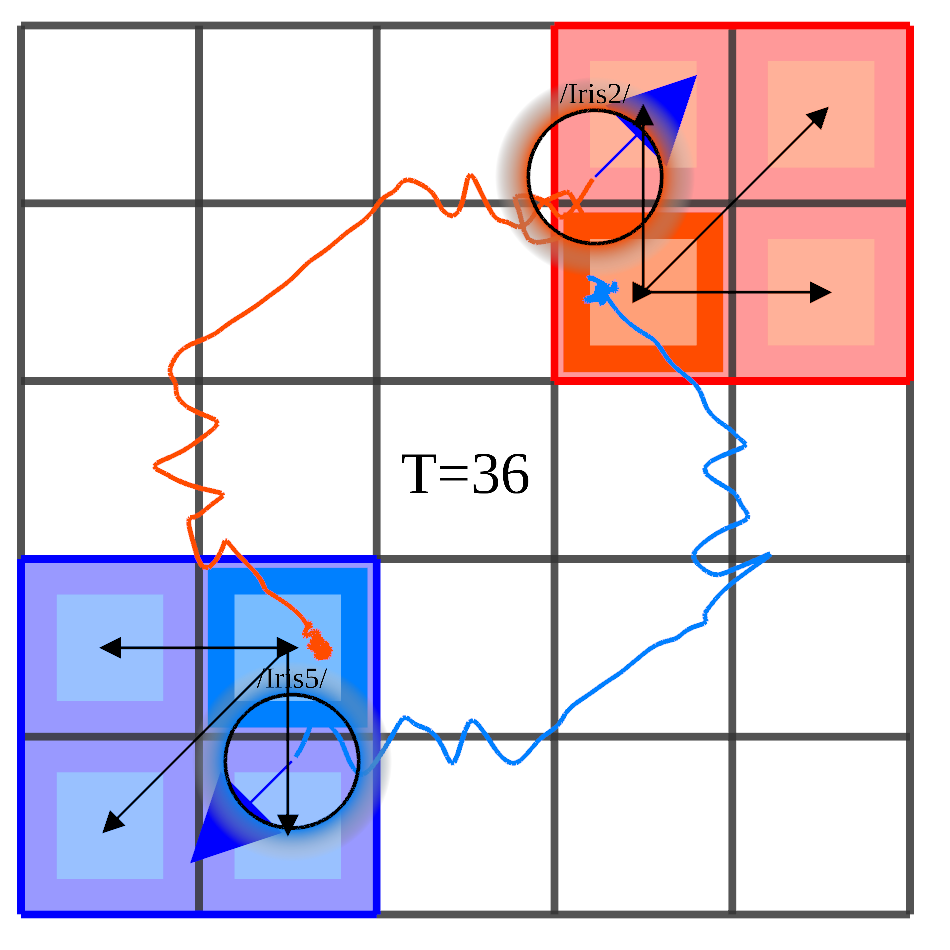
\includegraphics[width=\linewidth]{multi_ltl/multi11}
  \end{minipage} 
  \begin{minipage}{0.3\textwidth}
    \centering
    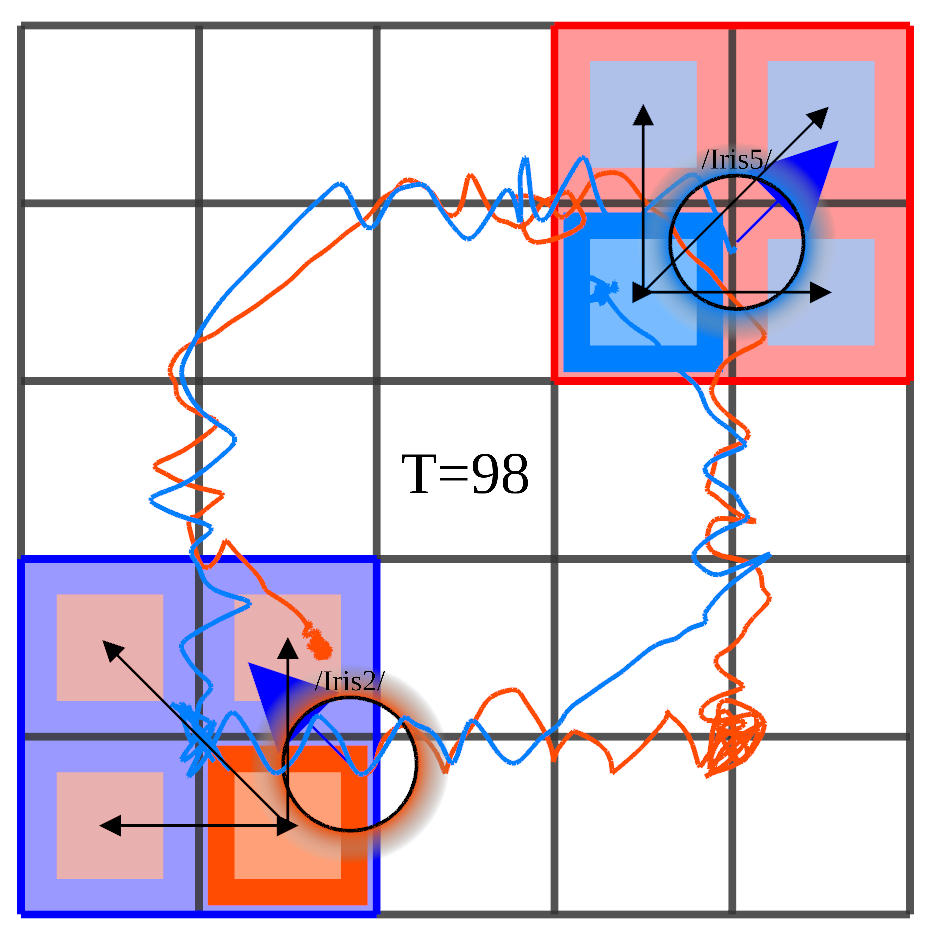
\includegraphics[width=\linewidth]{multi_ltl/multi12}
  \end{minipage} 

\caption{Run of the multiagent plan. Agent blue and red need to exchange position infinitely often. Cells in plain colors are the current state of the quadricopter. Cells in light color are the successors. Big blues arrows are the control action.}
\label{fig:multi}
\end{figure}


\section{Conclusion}
\comment{The strong cyclic planning method can be really effective in some case where the noise.
Conclude about when to use the strongly connected cyclic model.
How to choose the discretization.
Just accept the fact that there is no strong theoretical justifications?
Can I sort of generalize this method to a bigger class of model (not just the first integrator model)?
}
\comment{I must notice that the we are not using any optimal algorithm (DFS). This imply that the computing time are less than a relevant case scenario.}
